
\documentclass[aspectratio=169]{beamer}

% -------------------------------------------------
% Packages
% -------------------------------------------------
\usepackage{amsmath, amsfonts}
\usepackage{graphicx}
\usepackage{booktabs}
\usepackage{hyperref}
\usepackage{bm}
\usepackage{siunitx}
\usepackage{listings}

% Figure search paths (relative to tex/lectures/)
\graphicspath{{../figures/lectures/}{../figures/shared/}}

% -------------------------------------------------
% Notes (speaker notes)
% -------------------------------------------------
\usepackage{pgfpages}
% Uncomment ONE of these for speaker notes:
% \setbeameroption{show notes} % notes only (for printing notes)
% \setbeameroption{show notes on second screen=right} % slides + notes

% -------------------------------------------------
% TikZ
% -------------------------------------------------
\usepackage{tikz}
\usetikzlibrary{matrix, calc}
\usepackage{xcolor} % (tikz loads xcolor, but explicit is fine)
\usetikzlibrary{arrows.meta, decorations.pathreplacing}


% -------------------------------------------------
% Themes
%--------------------------------------------------
\usetheme{default}
\usecolortheme{default}
\setbeamertemplate{navigation symbols}{}

% -----------------------------
% Code formatting
% -----------------------------
\definecolor{codegray}{RGB}{245,245,245}

\lstset{
  backgroundcolor=\color{codegray},
  basicstyle=\ttfamily\small,
  frame=single,
  breaklines=true,
  showstringspaces=false
}

% --- Shortcuts ---
%\newcommand{\dd}{\,\mathrm{d}}
\newcommand{\Grad}{\nabla}
\newcommand{\Div}{\nabla\!\cdot}
\newcommand{\bx}{\bm{x}}
\newcommand{\bn}{\bm{n}}
\newcommand{\bq}{\bm{q}}

%==========================
% Flipbook macro (put in preamble or before frames)
%==========================
\newcommand{\GSFlipFrame}[2]{%
\begin{frame}{Gauss--Seidel sweep (current point $(#1,#2)$)}
\centering
\hspace{3.5cm}
\vspace{3cm}
\begin{tikzpicture}[scale=2.2, every node/.style={font=\small}]
  % -----------------------------
  % USER SETTINGS
  % -----------------------------
  \def\Nx{6}   % i = 0..Nx-1
  \def\Ny{4}   % j = 0..Ny-1

  % current stencil location (interior)
  \def\ci{#1}
  \def\cj{#2}

  % Point spacing
  \def\s{0.85}

  % -----------------------------
  % STYLES
  % -----------------------------
  \tikzset{
    gpG/.style={circle, fill=green!70!black, inner sep=1.1pt},
    gpR/.style={circle, fill=red!75!black,   inner sep=1.1pt},
    gpbG/.style={circle, fill=green!70!black, inner sep=1.5pt},
    gpbR/.style={circle, fill=red!75!black,   inner sep=1.5pt},
    gpc/.style={circle, fill=blue, inner sep=1.7pt},
    stline/.style={dashed, thick},
    labij/.style={font=\normalsize},
    labp/.style={font=\scriptsize, text=gray!70},
  }

  % -----------------------------
  % OUTER RECTANGLE (domain)
  % -----------------------------
  \draw[thick] (0,0) rectangle ({(\Nx-1)*\s},{(\Ny-1)*\s});

  % -----------------------------
  % GRID POINTS + LABELS
  % -----------------------------
  \foreach \j in {0,...,\numexpr\Ny-1\relax} {
    \foreach \i in {0,...,\numexpr\Nx-1\relax} {

      \pgfmathsetmacro{\x}{\i*\s}
      \pgfmathsetmacro{\y}{\j*\s}

      % global index p = i + j*Nx (as in your first figure)
      \pgfmathtruncatemacro{\p}{\i + \j*\Nx}

      % boundary?
      \pgfmathtruncatemacro{\isB}{ (\i==0) || (\i==\Nx-1) || (\j==0) || (\j==\Ny-1) }
      % current center?
      \pgfmathtruncatemacro{\isC}{ (\i==\ci) && (\j==\cj) }

      % "already updated" (GS ordering): j<cj OR (j==cj and i<ci)
      \pgfmathtruncatemacro{\isUpdated}{ (\j<\cj) || ((\j==\cj) && (\i<\ci)) }

      % FORCE left boundary (i==0) and bottom boundary (j==0) to be green
      \pgfmathtruncatemacro{\forceGreen}{ \isB }

      % decide color state:
      % - center: blue
      % - else green if forced green OR updated
      % - else red
      \ifnum\isC=1
        \node[gpc] (P\i\j) at (\x,\y) {};
      \else
        \pgfmathtruncatemacro{\isGreen}{ (\forceGreen==1) || (\isUpdated==1) }
        \ifnum\isB=1
          \ifnum\isGreen=1
            \node[gpbG] (P\i\j) at (\x,\y) {};
          \else
            \node[gpbR] (P\i\j) at (\x,\y) {};
          \fi
        \else
          \ifnum\isGreen=1
            \node[gpG] (P\i\j) at (\x,\y) {};
          \else
            \node[gpR] (P\i\j) at (\x,\y) {};
          \fi
        \fi
      \fi

      % Labels (i,j) above-right; p below-right
      \node[labij, anchor=south west] at (\x+0.05,\y+0.05) {$(\i,\j)$};
      \node[labp,  anchor=north west] at (\x+0.05,\y-0.05) {$\p$};
    }
  }

  % -----------------------------
  % 5-POINT STENCIL (dashed)
  % -----------------------------
  \pgfmathsetmacro{\xc}{\ci*\s}
  \pgfmathsetmacro{\yc}{\cj*\s}

  \draw[stline] (\xc,\yc) -- ({(\ci+1)*\s},\yc);
  \draw[stline] (\xc,\yc) -- ({(\ci-1)*\s},\yc);
  \draw[stline] (\xc,\yc) -- (\xc,{(\cj+1)*\s});
  \draw[stline] (\xc,\yc) -- (\xc,{(\cj-1)*\s});

  % Mapping note
  %\node[font=\scriptsize, align=left] at ({(1)*\s+1.65},{(0)*\s-0.55})
  %{$p = i + j\,N_x$};
\end{tikzpicture}
\end{frame}%
}











\title[Divergence Theorem via 1D Fin]{Divergence Theorem via 1D Heat Conduction\\(Constant Cross Section)}
\author{MMAE 450}
\date{}

\newcommand{\dd}{\,\mathrm{d}}
\newcommand{\vect}[1]{\bm{#1}}

\begin{document}

% -------------------- Slide 1 --------------------
\begin{frame}
\titlepage
\end{frame}

% -------------------- Slide 2 --------------------
\begin{frame}{Big Idea}
\begin{block}{Core principle}
Local conservation laws, when integrated over a domain, become global balance laws.
\end{block}

\begin{itemize}
  \item Boundary view: add what crosses the boundary
  \item Interior view: add what is created or destroyed inside
\end{itemize}

\vspace{0.5em}
These two viewpoints are equivalent.
\end{frame}

% -------------------- Slide 3 --------------------
\begin{frame}{1D Fin Model}
\begin{itemize}
  \item Fin along \(x \in [0,L]\)
  \item Constant cross-sectional area \(A\)
  \item Heat flux \(q(x)\) [W/m\(^2\)]
  \item Steady state
  \item No internal heat generation
\end{itemize}

\begin{block}{Goal}
Derive the local and global energy balance from first principles.
\end{block}
\end{frame}

% -------------------- Slide 4 --------------------
\begin{frame}{Control Volume in the Fin}
\centering
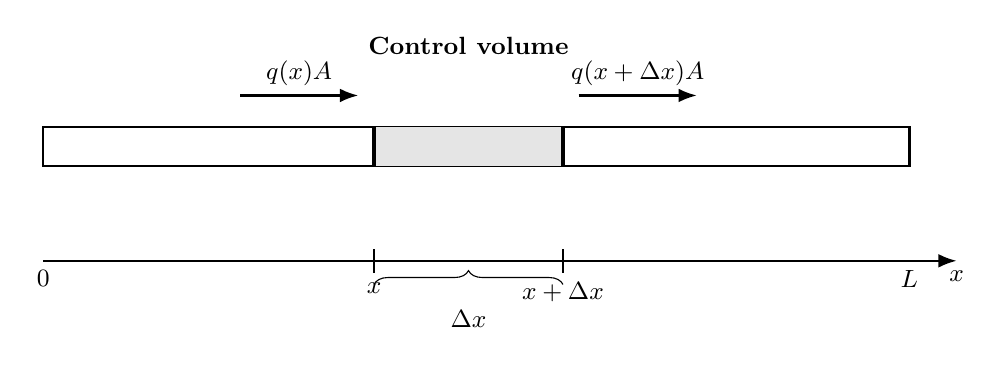
\begin{tikzpicture}[x=1cm,y=1cm,>=Latex, font=\small]
  \def\L{11.0}
  \def\h{0.5}
  \def\xa{4.2}
  \def\xb{6.6}

  % Axis
  \draw[->, thick] (0,-1.2) -- (\L+0.6,-1.2) node[below] {$x$};
  \node[below] at (0,-1.2) {$0$};
  \node[below] at (\L,-1.2) {$L$};

  % Fin
  \draw[thick] (0,0) rectangle (\L,\h);

  % Control volume
  \fill[black!10] (\xa,0) rectangle (\xb,\h);
  \draw[very thick] (\xa,0) -- (\xa,\h);
  \draw[very thick] (\xb,0) -- (\xb,\h);

  % Labels
  \draw[thick] (\xa,-1.05) -- (\xa,-1.35);
  \draw[thick] (\xb,-1.05) -- (\xb,-1.35);
  \node[below] at (\xa,-1.35) {$x$};
  \node[below] at (\xb,-1.35) {$x+\Delta x$};

  \draw[decorate, decoration={brace, amplitude=5pt}] (\xa,-1.5) -- (\xb,-1.5)
    node[midway, below=6pt] {$\Delta x$};

  % Flux arrows
  \draw[->, thick] (\xa-1.7,0.9) -- (\xa-0.2,0.9);
  \node[above] at (\xa-0.95,0.9) {$q(x)A$};

  \draw[->, thick] (\xb+0.2,0.9) -- (\xb+1.7,0.9);
  \node[above] at (\xb+0.95,0.9) {$q(x+\Delta x)A$};

  \node[above] at ({0.5*(\xa+\xb)},1.3) {\textbf{Control volume}};
\end{tikzpicture}
\end{frame}

% -------------------- Slide 5 --------------------
\begin{frame}{Local Energy Balance (No Generation)}
On the segment \([x, x+\Delta x]\), steady state with no generation:
\[
q(x)A - q(x+\Delta x)A = 0
\]

Divide by \(A\,\Delta x\) and take the limit \(\Delta x \to 0\):
\[
\frac{q(x+\Delta x)-q(x)}{\Delta x} = 0
\quad\Rightarrow\quad
\frac{dq}{dx} = 0
\]

\begin{block}{Interpretation}
The heat flux is spatially constant when no energy is generated.
\end{block}
\end{frame}

% -------------------- Slide 6 --------------------
\begin{frame}{From Local to Global Balance}
Integrate the local conservation law over \([0,L]\):
\[
\int_0^L \frac{dq}{dx}\,dx = 0
\]

Apply the Fundamental Theorem of Calculus:
\[
q(L) - q(0) = 0
\]

\begin{block}{Boundary heat-rate balance}
Multiplying by the area gives
\[
q(0)A = q(L)A
\]
\end{block}
\end{frame}

% -------------------- Slide 7 --------------------
\begin{frame}{Local Balance with a Source Term}
Now include volumetric heat generation \(S(x)\) [W/m\(^3\)].

Energy balance on \([x,x+\Delta x]\):
\[
q(x)A - q(x+\Delta x)A + S(x)\,A\,\Delta x = 0
\]

Divide by \(A\,\Delta x\) and take the limit:
\[
-\frac{dq}{dx} + S(x) = 0
\]

\begin{block}{Local conservation law}
Divergence of heat flux balances internal generation.
\end{block}
\end{frame}

% -------------------- Slide 8 --------------------
\begin{frame}{Global Balance with Sources}
Integrate the local equation over \([0,L]\):
\[
\int_0^L \left(-\frac{dq}{dx} + S(x)\right)\,dx = 0
\]

\[
-\big(q(L)-q(0)\big) + \int_0^L S(x)\,dx = 0
\]

Multiply by the area:
\[
q(0)A - q(L)A + \int_0^L S(x)\,A\,dx = 0
\]

\begin{block}{Meaning}
\(\text{in} - \text{out} + \text{generated} = 0\)
\end{block}
\end{frame}

% -------------------- Slide 9 --------------------
\begin{frame}{Divergence Theorem (Heat)}
In three dimensions, let \(\vect{q}(\vect{x})\) be the heat flux vector.

\[
-\nabla \cdot \vect{q} + S = 0
\]

Integrating over a volume \(V\):
\[
\int_V \nabla\cdot \vect{q}\,dV
=
\int_{\Gamma} \vect{q}\cdot \vect{n}\,dS
\]

\begin{block}{Key idea}
Divergence converts surface flux into a volumetric density.
\end{block}
\end{frame}

% -------------------- Slide 10 --------------------
\begin{frame}{Exact Analogy: Stress Divergence}
Replace heat flux with the Cauchy stress tensor \(\boldsymbol{\sigma}\).

\[
\int_V \nabla\cdot \boldsymbol{\sigma}\,dV
=
\int_{\Gamma} \boldsymbol{\sigma}\vect{n}\,dS
\]

Linear momentum balance:
\[
\nabla\cdot \boldsymbol{\sigma} + \vect{b} = \rho \vect{a}
\]

\begin{itemize}
  \item \(\nabla\cdot \boldsymbol{\sigma}\): internal force per unit volume
  \item \(\vect{b}\): body force density
\end{itemize}

\begin{block}{One-sentence takeaway}
Divergence turns boundary interactions into volume forces.
\end{block}
\end{frame}

% -------------------- Slide 11 --------------------
\begin{frame}{Wrap-Up}
\begin{itemize}
  \item Start from conservation on an infinitesimal segment
  \item Divide by volume to obtain a local law
  \item Integrate to recover the global balance
  \item Same structure appears in heat, fluids, and solids
\end{itemize}

\begin{block}{Exit question}
If \(S=0\), what must be true of the boundary heat fluxes?
\end{block}
\end{frame}

\end{document}
